% This example is meant to be compiled with lualatex or xelatex
% The theme itself also supports pdflatex
\PassOptionsToPackage{unicode}{hyperref}
\documentclass[aspectratio=1610, 9pt]{beamer}

% Load packages you need here
\usepackage{polyglossia}
\setmainlanguage{german}

\usepackage{csquotes}


\usepackage{amsmath}
\usepackage{amssymb}
\usepackage{mathtools}

\usepackage{hyperref}
\usepackage{bookmark}
\usepackage{wrapfig}
\usepackage{lipsum}
%\usepackage{minipage}

% load the theme after all packages

\usetheme[
  %showtotalframes, % show total number of frames in the footline
  % dark, % optional dark theme, uncomment to use
]{tudo}

% Put settings here, like
\unimathsetup{
  math-style=ISO,
  bold-style=ISO,
  nabla=upright,
  partial=upright,
  mathrm=sym,
}

\title{Stochastische Thermodynamik II: Entropieproduktion, Thermodynamische Unschärferelation}
\author[S.~Öz]{Selin Öz}
\institute{AG Kierfeld\\ Fakultät Physik}
%\titlegraphic{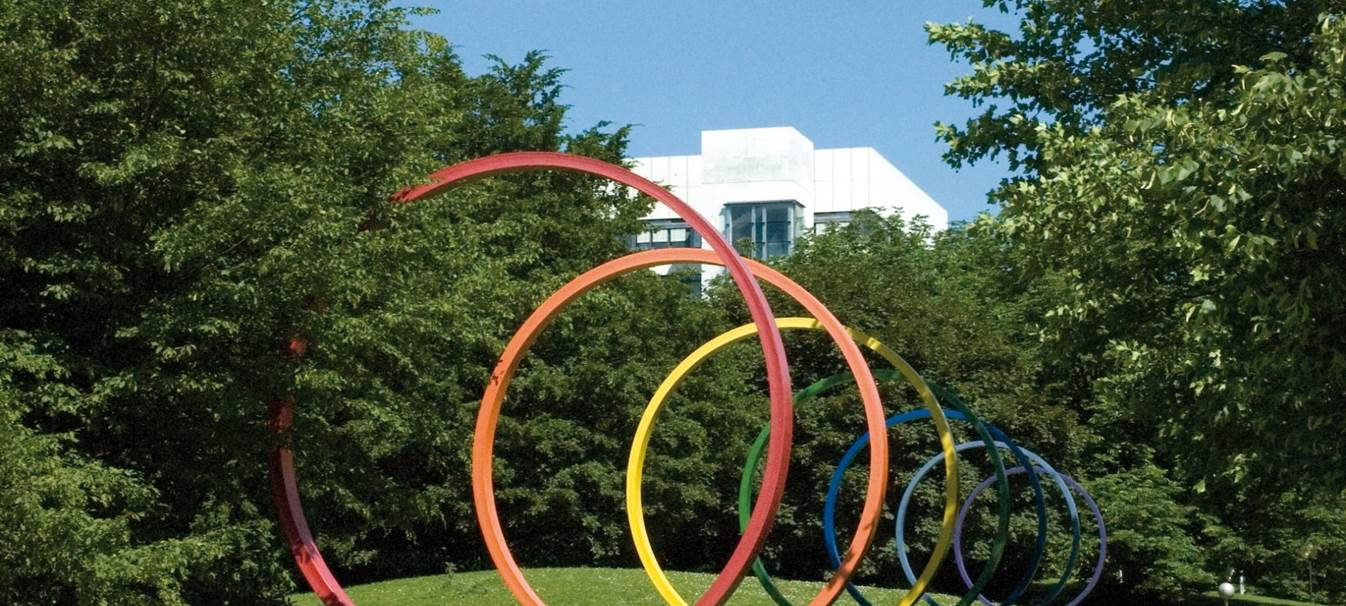
\includegraphics[width=0.7\textwidth]{images/tudo-title-2.jpg}}


\begin{document}

\maketitle


\begin{frame}{Einführung}
  \tableofcontents
\end{frame}

\section{Mesostates}
\begin{frame}{Mesostates}%%%%%%%%%%%%%%%%%%%%%%%%%%%%%%%%%%%%%%%%%%%%%%%%%%%%%%%%%%%%%%%%%%%%%%%%%%%%%%%%%%%%%%%%%%%%%%%%%%%%%%%%%%%%%%%%%%%%%%%%%%%%%%%%%%%%%%%%%5
    \begin{itemize}
      \item \textbf{Microstate}  $\xi$ mit Energie $ H \left(\xi \right) $ eines geschlossenen Geleichgewichtssystem im Kontakt mit Wärmebad mit der inversen Temperatur $\beta$
      \item Aus der statistischen Thermodynamik sind die \textbf{Freie Energie} $F$, \textbf{innere Energie} $U$ und \textbf{Entropie} $S$ bekannt 
      \begin{equation*}
        F=-(1 / \beta )\ln\sum_{\xi}\exp[-\beta H(\xi)], \quad U=\partial_{\beta}(\beta F), \quad S = \beta^2 \partial_\beta F
      \end{equation*}
      \hspace{-20pt}
      \begin{minipage}[t]{0.7\textwidth}
        \begin{itemize}
        \item Microstates $\xi$ gehören einem \textbf{Mesostate} $I$. Die Wahrscheinlichkeit für den Mesostate $I$
        \begin{equation*}
        P_I=  \sum_{\xi \in I} \exp[-\beta \left( H(\xi) - F\right) ] \equiv \exp[-\beta \left( F_I - F\right) ]
        \end{equation*}
        \end{itemize}
      \end{minipage}
      \hfill
      \begin{minipage}{0.25\textwidth}
        \begin{center}
          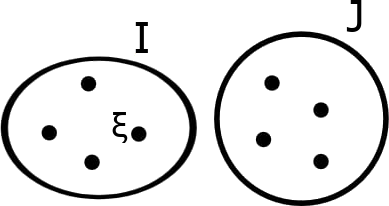
\includegraphics{images/mesostates.png}
        \end{center}
      \end{minipage}
      \item Die bedingte Wahrscheinlichkeit des Microstates $\xi$
      \begin{equation*}
      P(\xi|I)= \exp[-\beta \left( H(\xi) - F\right) ] / P_I  = \exp[-\beta \left( H(\xi) - F_I\right) ]
      \end{equation*}
      \item Daraus folgen für die Freie Energie $F_I$, innere Energie $U_I$ und Entropie $S_I$ 
      \begin{equation*}
        F_I=-(1 / \beta )\ln\sum_{\xi \in I }\exp[-\beta H(\xi)], \quad U_I=\partial_{\beta}(\beta F_I), \quad S_I = \beta^2 \partial_\beta F = - \sum_{\xi \in I }   P(\xi|I) \ln   P(\xi|I)
      \end{equation*}
    \end{itemize}
\end{frame}%%%%%%%%%%%%%%%%%%%%%%%%%%%%%%%%%%%%%%%%%%%%%%%%%%%%%%%%%%%%%%%%%%%%%%%%%%%%%%%%%%%%%%%%%%%%%%%%%%%%%%%%%%%%%%%%%%%%%%%%%%%%%%%%%%%%%%%%%%%%%%%

\begin{frame}{}%%%%%%%%%%%%%%%%%%%%%%%%%%%%%%%%%%%%%%%%%%%%%%%%%%%%%%%%%%%%%%%%%%%%%%%%%%%%%%%%%%%%%%%%%%%%%%%%%%%%%%%%%%%%%%%%%%%%%%%%%%%%%%%%%%%%%%%%%5
  \begin{itemize}
    \item die freie Energie-Differenz zwischen den Mesostates $I$ und $J$
    \begin{equation*}
      \Delta_{IJ}F = F_J - F_I = - (1 / \beta )\ln[P_J / P_I]
    \end{equation*}
    \item aus der freien Energie-Differenz lässt sich die \textbf{detailed balance condition} ableiten
    \begin{equation}
        K_{I J} / K_{ J I} = \exp[-\beta \Delta_{IJ}F ],
    \end{equation}
    wobei $ K_{I J} = \partial_t P(J,t'|I,t)_{t'=t}$ die Übergangsrate ist
    \item Wenn die Microstate-Dynamik schneller ist als die, der Mesostates,
    können die Übergangsraten unhabhänig davon, wie lange man sich in einem Zustand befindet, betrachtet werden.
    Die zeitliche Entwicklung der Wahrscheinlichkeit wird mit der \textbf{Master equation} beschrieben
    \begin{equation}
      \partial_t P_I(t) = \sum_J[ P_J(t)K_{J I}- P_I(t)K_{I J}]
    \end{equation}
  \end{itemize}
\end{frame}%%%%%%%%%%%%%%%%%%%%%%%%%%%%%%%%%%%%%%%%%%%%%%%%%%%%%%%%%%%%%%%%%%%%%%%%%%%%%%%%%%%%%%%%%%%%%%%%%%%%%%%%%%%%%%%%%%%%%%%%%%%%%%%%%%%%%%%%%%%%%%%

\section{Entropieproduktion für geschlossene Systeme}
\begin{frame}{Entropieproduktion entlang einer Trajektorie}
  \begin{itemize}
    \item Die \textbf{totale Entropieproduktion} entlang einer Trajektorie ein Maß für eine gebrochene Zeit-Symmetrie
    \begin{equation*}
      \Delta S_\text{tot}[I(t)] \equiv  \ln \left(P[I(t)]/ \tilde{P}[\tilde{I}(t)] \right) 
    \end{equation*}
    mit $\tilde{I}(t)  \equiv  I( \Tau -t)$ 
    \item mit der \textbf{Master equation} für die explitziete P[I(t)], lässt sich die Entropieproduktion in drei Teile teilen
    \begin{equation*}
      \Delta S_\text{tot}[I(t)] = \beta Q[I(t)] + \Delta S[I(t)] + \Delta S_\text{sto}[I(t)]
    \end{equation*}
    \begin{itemize}
      \item $\beta Q[I(t)] = -\beta \left(U_{I^\Tau}- U_{I^0} \right)$ ist die Entropieänderung im Wärmebad durch dissipierte Wärme 
      \item $\Delta S[I(t)] = S_{I^\Tau}- S_{I^0} $ ist Änderung der intrinsischen Entropie, wird oft vernachlässigt
      \item $S_\text{sto}[I(t)]= - \ln P_{I(t)}(t)$ ist die Änderung der Stochastischen Entropie
    \end{itemize}
  \end{itemize}
\end{frame}

\begin{frame}{Entropieproduktion im Esemble}%%%%%%%%%%%%%%%%%%%%%%%%%%%%%%%%%%%%%%%%%%%%%%%%%%%%%%%%%%%%%%%%%%%%%%%%%%%%%%%%%%%%%%%%%%%%%%%%%%%%%%%%%%%%%5
  \begin{itemize}
    \item Die Entropieproduktion zwischen zwei Mesostates $I$ und $I$ setzt sich analog zusammen
    \begin{equation*}
      \Delta_{IJ} S[I(t)] = \beta Q_{IJ} + \Delta_{IJ} S^\text{sys} = \ln[P_I(t)K_{IJ}/P_J(t)K_{JI}]
    \end{equation*}
    \begin{itemize}
      \item $\beta Q_{IJ}= -\beta \left(U_{I}- U_{J} \right)$ ist die Entropieänderung im Wärmebad durch dissipierte Wärme 
      \item $ S^\text{sys}= S_{I(t)}  - \ln P_{I(t)}(t)$, $S_{I(t)}$ ist die intrinsische Entropie 
    \end{itemize}
    \item die Entropieproduktion zwischen zwei Mesostates gemittelt über die Anzahl der Wechsel $n_{IJ}$ von $I$ zu $I$  in der Zeit $ \Tau$ ist die totale Entropieproduktion
    \begin{equation*}
      \Delta S_\text{tot}[I(t)]= \sum_{IJ} n_{IJ}  \Delta_{IJ} S[I(t)] = \sum_{IJ} n_{IJ}  \ln[P_I(t)K_{IJ}/P_J(t)K_{JI}]
    \end{equation*}
    \item die mittlere Entropieproduktionsrate 
    \begin{equation*}
    <\dot{s}_\text{tot}> = \sum_{IJ} P_I(t)K_{IJ} \Delta_{IJ} S[I(t)] = \sum_{I<J} [P_I(t)K_{IJ}-P_J(t)K_{JI}] \ln[P_I(t)K_{IJ}/P_J(t)K_{JI}] \geq 0
    \end{equation*}
    \item \textbf{ integral fluctuation theorem} für totale Entropieproduktion
    \begin{equation*}
      <\exp[-\Delta S_\text{tot}]> = 1
    \end{equation*}
  \end{itemize}
\end{frame}%%%%%%%%%%%%%%%%%%%%%%%%%%%%%%%%%%%%%%%%%%%%%%%%%%%%%%%%%%%%%%%%%%%%%%%%%%%%%%%%%%%%%%%%%%%%%%%%%%%%%

\begin{frame}{Entropieproduktion durch Phänomenologie}
  \begin{minipage}{0.5\textwidth}
    \begin{itemize}
      \item Strom $J_{ij} = K_{ij} P_j - K_{ji} P_i$
      \item zu jeden Kreis $C_k$ gehört eine Affinität $A_{ij} = \ln K_{ij} P_j / K_{ji} P_i$
      \item Entropieproduktionsrate $\sigma = \sum_{i,j} J_{ij} A_{ij }= \sum_{I<J} [P_I(t)K_{IJ}-P_J(t)K_{JI}] \ln[P_I(t)K_{IJ}/P_J(t)K_{JI}] $
    \end{itemize}
  \end{minipage}
\begin{minipage}{0.4\textwidth}
    \begin{center}
      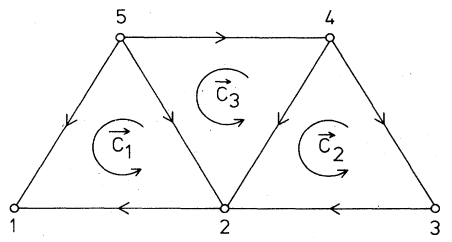
\includegraphics[width=\textwidth]{images/circle.png}
    \end{center}
  \end{minipage}
\end{frame}



\section{Entropieproduktion für offene Systeme}

\begin{frame}{Entropieproduktion für offene Systeme}%%%%%%%%%%%%%%%%%%%%%%%%%%%%%%%%%%%%%%%%%%%%%%%%%%%%%%%%%%%%%%%%%%%%%%%%%%%%%%%%%%%%%%%%%%%%%%%%%%%%%%%%%%%%%%
  \begin{itemize}
    \item System wird aufgeteilt in
    \begin{itemize}
      \item Kern-System
      \item Umgebende-Lösung, die als Teilchen-Reservoir dient, und externe machanische Arbeit liefert
    \end{itemize}
    \item Die \textbf{detailed balance condition} wird zu
    \begin{equation}
      K_{I J} / K_{ J I} = \exp[-\beta \Delta_{IJ}F - \sum_\alpha \mu^\alpha d_{IJ}^\alpha + f d_{IJ}],
  \end{equation}
  wobei $d_{IJ}^\alpha >0$ heißt, dass Teilchen der Sorte $\alpha$ vom chemische Potential $\mu^\alpha$ abgegeben werden,
  $f d_{IJ}$ ist die Arbeit, die von der Kraft $f$ entlang der Länge $d_{IJ}$ verrichtet wird 
  \item Die Master equation beschreibt die Wahrscheinlichkeien des Kern-Systems
  \begin{equation}
    \partial_t P_I(t) = \sum_J[ P_J(t)K_{J I}- P_I(t)K_{I J}]
  \end{equation}
\end{itemize}  
\end{frame}


\begin{frame}%%%%%%%%%%%%%%%%%%%%%%%%%%%%%%%%%%%%
  \begin{itemize}
  \item Der erste Haupsatzt für die Trajektorie $I \rightarrow J $
  \begin{equation*}
    \Delta_{IJ} U +  \Delta_{IJ} U^\text{sol} + W^\text{out}_{IJ} = - Q_{{IjJ}}
  \end{equation*}
    \item  Zur Entropieänderung des Systems kommt nur die intrinsische Entropieänderung der Umgebundslösung
    \begin{equation*}
      \Delta_{IJ}S^\text{sys}(t)= \Delta_{IJ}S + \Delta_{IJ}S^\text{sol}  - \ln P_I / P_J
    \end{equation*}
    \item Die totale Entropieänderung ist denach
    \begin{equation*}
      \Delta_{IJ} S(t) = \beta Q_{IJ} + \Delta_{IJ} S^\text{sys}(t) = \ln[P_I(t)K_{IJ}/P_J(t)K_{JI}]
    \end{equation*}
    \item der zweite Hauptsatz auf Ensemble-Level
    \begin{equation*}
      <\dot{s}_\text{tot}> = \sum_{IJ} P_I(t)K_{IJ} \Delta_{IJ} S[I(t)] = \sum_{I<J} [P_I(t)K_{IJ}-P_J(t)K_{JI}] \ln[P_I(t)K_{IJ}/P_J(t)K_{JI}] \geq 0
    \end{equation*}
  \end{itemize}
\end{frame}%%%%%%%%%%%%%%%%%%%%%%%%%%%%%%%%%%%%%%%%%%%%%%%%%%%%%%%%%%%%%%%%%%%%%%%%%%%%%%%%%%%%%%%%%%%%%%%%%%%%%%%%%%%%%%%%%%%%%%%%%%%%%%%%%%%%%%%%%%%%%%%%%%%%%%%%%

\begin{frame}{Beispiel: Motorproteine}
  \begin{minipage}{0.38\textwidth}
    Ein Motor mit zwei Kopfen, der mit Hydrolyse von ATP betrieben wird (Kinesin)
    \begin{itemize}
     \item[(1\rightarrow 2)] ATP bindet ans Molekühl
     \item[(2\rightarrow 3)] ATP-Hydrolyse zu ADP und anorganisches Phosphat, vorderer Kopf macht Schritt
     \item[(3\rightarrow 1)] ADP löst sich, hinterer Kopf macht Schritt
    \end{itemize}

    \begin{itemize}
      \item $\alpha= T, D , P$ für ATP, ADP, Phosphat 
      \item $d^T_{12}=1$, $d^P_{23}=1$, $d^D_{31}=1$, und $d^\alpha_{IJ}=0$
      \item $d_{23} = d_{31} = d/2$, $d_{12} = 0$, and $d_{JI} = −d_{IJ}$
      \item Die Rückraten $K_{21}$, $K_{32}$ und $K_{13}$ sind kleiner als $K_{12}$, $K_{23}$ und $K_{31}$
     \end{itemize}

 \end{minipage}
    \begin{minipage}{0.6\textwidth}
      \begin{center}
        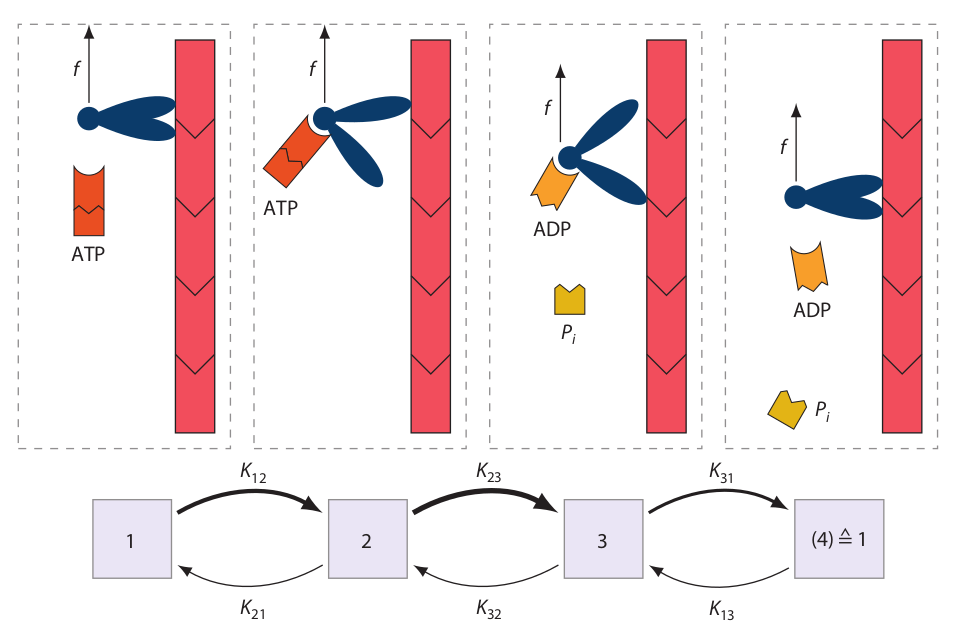
\includegraphics[width=\textwidth]{images/motor.png}
      \end{center}
    \end{minipage}
\end{frame}


\begin{frame}{Unschärferelation anhand eines Beispiels}

\begin{minipage}{0.5\textwidth}

Asymetrischer radom walk
\begin{itemize}
  \item mittlere Position $<n>= j \Tau$ nach Zeit $\Tau$
  \item mittlere Strom $j = K_+ - K_-$
  \item Diffusionkoeffizient $D = <(n-<n>)^2> / 2 \Tau  = (K_+ + K_-)/2$
  \item mittlere Entropieproduktion $\sigma= (K_+ - K_-) \ln K_+ / K_-$
\end{itemize}

\begin{equation*}
\sigma \geq j^2 / D 
\end{equation*}

\begin{equation*}
  (K_+ - K_-) \ln K_+ / K_- \geq 2 (K_+ - K_-)^2 / (K_+ + K_-)
\end{equation*}
für $K_+  \geq K_-$

\end{minipage}
\begin{minipage}{0.49\textwidth}
  \begin{center}
    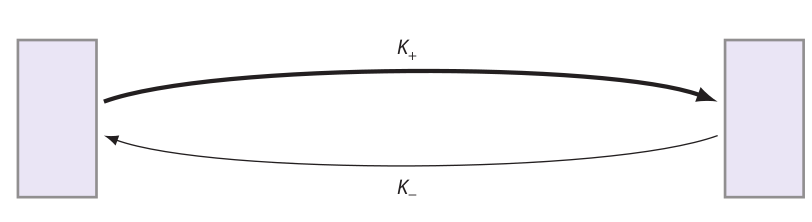
\includegraphics[width=\textwidth]{images/random.png}
  \end{center}
\end{minipage}
\end{frame}

\section{Unschärferelation}
\begin{frame}
  \begin{block}{Unschärferelation allgemein}
    \begin{equation*}
      \sigma \geq j^2 / D 
      \end{equation*}

      \begin{center}
        mit $j= <X(\Tau)>/\Tau$ und $D= \displaystyle{\lim_{\Tau \to \infty}} <X^2(\Tau)> - <X(\Tau)>^2 / 2 \Tau$ und $X = \sum_{IJ} d_{IJ} n_{IJ}(\Tau)$ 
        mit $d_{IJ} = - d_{JI}$
      \end{center}

  \end{block}
  Herleitung:

  "Level 2.5 large deviations for continuous-time Markov processes" rate function $I$, gibt ein asyomptotisches Limit für eine Wahrscheinlichkeit für Fluktuationen
  \begin{equation*}
    -1 / T \ln P(p, j) = I(p,j)
  \end{equation*}
  $I(p,j)$ wird die Fluktuationen der empirischen Stroms $j$ und der empirischen Wahrscheinlichkeitsdichte $p$, $I(p,j)$ ist bekannt
  \begin{equation*}
     I(p,j) = \sum_{y<z} \Psi(j(y,z)), j^p(y,z), a^p(y,z)
  \end{equation*}
  mit $\Psi = \left[ j \left( (\text{arcsinh}(j/a)- \text{arcsinh}(\bar{j}/a) )\right) - \left( \sqrt{ a^2 + j^2}- \sqrt{ a^2 + \bar{j}^2}\right) \right]$, 
  $\bar{j}= j / j^p$,
  $j^p = p(y)r(y,z)- p(z)r(z,y)$ und 
  $a^p = \sqrt{p(y)p(z)r(y,z)r(z,y)}$
\end{frame}


\begin{frame}
  $\Psi$ wird bis zur zweiten Ordung getaylort
  \begin{equation*}
    \Psi \leq \Psi_\text{quadratisch} = \frac{(j- \bar{j})^2}{4 \bar{j}^2} \left( 2 \bar{j }  \text{ arcsinh}(\bar{j} / a )\right)
  \end{equation*}

  $\Psi$ wird über die Entropie $S = \ln\frac{p(y)r(y,z)}{p(z)r(z,y)}$ ausgedrückt
  \begin{equation*}
    \Psi \leq \Psi_\text{quadratisch} = \frac{(\bar{j} -1 )^2 \sigma^p }{4 } 
  \end{equation*}
  mit $\sigma^p = j^p S $
   
  mit $\Psi$ wird $I(p,j)$ berechnet
  \begin{equation*}
    I(p,j)  \leq I_\text{quadratisch} (p,j) = \sum_{y<z} \frac{\sigma^p }{4  j^p(y,z)^2} (j(y,z) - j^p(y,z))^2 
  \end{equation*}

  $j$ wird mit $d$ projeziert: $j_d = j\cdot d$

  \begin{equation*}
    I(p,j)  \leq I_\text{quadratisch} (p,j) = \frac{ (j_d - j^p(y,z))^2}{4  j^p(y,z)^2}  \sum_{y<z} \sigma^p 
  \end{equation*}

  mit $\text{var}(j_d) = 1 / I''$

  \begin{equation*}
      \frac{ 2(j_d)^2 }{\text{var}(j_d)} \leq \sum_{y<z} \sigma^p 
  \end{equation*}

  Als letzes wird $j_d \to  X $ ersetzt


\end{frame}



\begin{frame}{Thermodynamische Kosten und Unsicherheit}
  Aus der Unschärferelation lassen dich die \textbf{thermodynamic uncertainty relation} herleiten
  \begin{itemize}
    \item die Unsicherheit $\epsilon^2 \equiv <(n-<n>)^2> / <n>^2 = 2 D / (j^2 \Tau )$ für $\Tau \to \infty$ mit $<n>= j \Tau$
    \item die thermodynamische Kosten $C= \sigma \Tau / \beta$
  \end{itemize}
  \begin{align*}
    \sigma &\geq j^2 / D  &|\cdot \Tau / \beta \\
    \sigma  \Tau / \beta &\geq j^2 / D  \Tau / \beta & \\
  \end{align*}

  \begin{block}{thermodynamic uncertainty relation}
    \begin{equation*} 
      C \geq 2 / \beta / \epsilon^2 
    \end{equation*}
  \end{block}
\end{frame}

\begin{frame}{Abschätzung des Wirkungsgrad molekular Motoren}
  \begin{itemize}
    \item die Input-Leitung $P^\text{in}$
    \item die Output-Leitung $P^\text{out}= f v $, $f$ ist die Kraft, $v$ die Geschwindigkeit
    \item die mittlere Entropieproduktionsrate ist $\sigma = \beta( P^\text{in} - P^\text{out})$
    \item der Wirkungsgrad ist über $\eta = P^\text{out} / P^\text{in}$ definiert
  \end{itemize}
  \begin{block}{obere Grenze des Wirkungsgrads}
    \begin{equation*} 
     \eta = \frac{P^\text{out}}{P^\text{in}} =  \frac{P^\text{out}}{P^\text{out} + \sigma / \beta } =  \frac{ f v }{f v+ \sigma / \beta }
     \leq \frac{ 1}{1+ v / (D f \beta) }
    \end{equation*}
  \end{block}
\end{frame}

\begin{frame}{Wirkungsgrad von Kinesin}
  
  \begin{minipage}{0.5\textwidth}
    Ein Kinesin wird eine einem Bead verbundenm, dass in einer optischen Falle ist.
    Gemessen werden
    \begin{itemize}
      \item Geschwindigkeit $v$
      \item Diffusionskonstante $D$
      \item randomness Parameter $r= 2 D / v d $, d entspricht Motorschrittlänge
    \end{itemize}

    \begin{equation*}
      \eta \leq  \frac{ r}{ r + 2 / f d }
    \end{equation*}

  \end{minipage}
\begin{minipage}{0.4\textwidth}
    \begin{center}
      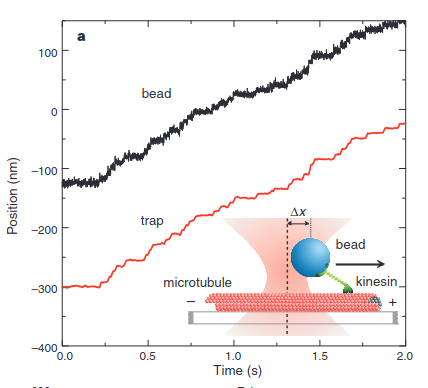
\includegraphics[width=\textwidth]{images/kinesin_pos.png}
    \end{center}
  \end{minipage}

\end{frame}

\begin{frame}
  
  \begin{minipage}{0.59\textwidth}
    \begin{center}
      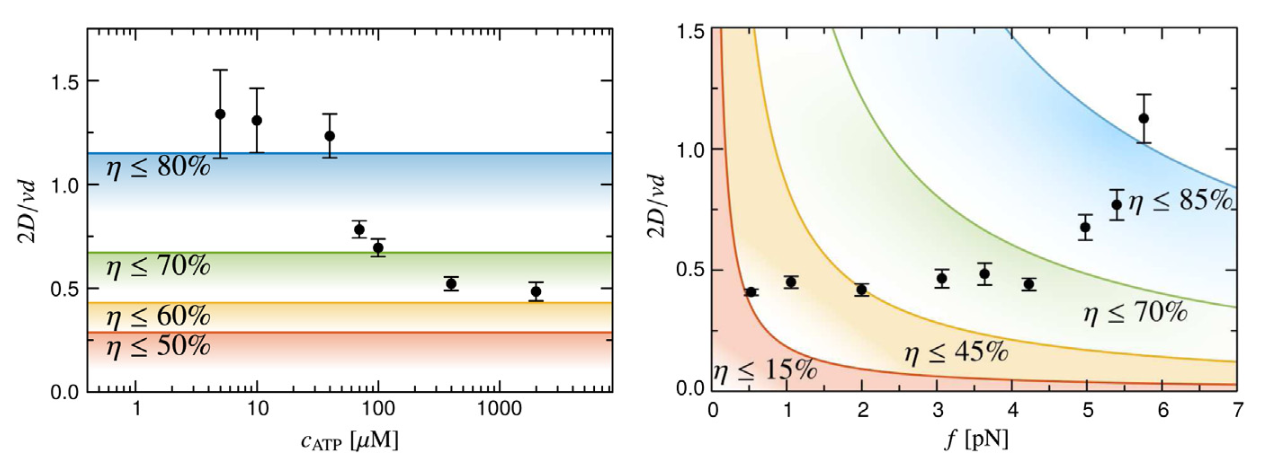
\includegraphics[width=\textwidth]{images/kinesin_r.png}
    \end{center}
  \end{minipage}
\begin{minipage}{0.4\textwidth}
    \begin{center}
      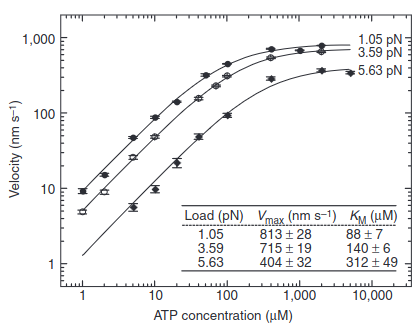
\includegraphics[width=\textwidth]{images/kinesin_v.png}
    \end{center}
  \end{minipage}

\end{frame}

\begin{frame}{Zusammenfassung}
  Entropieproduktion
  \begin{itemize}
    \item Esemble-Beschreibung und Trajektorien-Beschreibung sind equvalent 
    \item Totaler Entropieproduktion setzt sich aus drei Teilen zusammen (Änderung im Bad, intrinsische Entropie und stochstische Entropie)
  \end{itemize}
Unschärferelation
\begin{itemize}
  \item nutzen Entropieproduktion 
  \item können Aussagen über Ströme, Unschärfekosten und Wirkungsgrade treffen
\end{itemize}
\end{frame}
\end{document}

